\documentclass[a4paper]{jpconf}
\usepackage{graphicx}
%\usepackage{subcaption}

\newcommand{\GeV}{\ensuremath{\mathrm{\:GeV}}}
\newcommand{\TeV}{\ensuremath{\mathrm{\:TeV}}}
\newcommand{\pythia}{\textsc{Pythia8}}
\newcommand{\herwig}{\textsc{Herwig7}}
\newcommand{\chhh}{\ensuremath{\kappa_{\lambda}}}


\begin{document}

\title{Trilinear Higgs boson coupling variations for di-Higgs production with full NLO QCD predictions in \texttt{Powheg}}

\author{G.~Heinrich$^1$, S.~Jones$^2$, M.~Kerner$^3$, G.~Luisoni$^1$ and L.~Scyboz$^1$}

\address{$^1$ Max-Planck-Institut f\"ur Physik (Werner-Heisenberg-Institut), F\"ohringer Ring 6, 80805 M\"unchen, Germany}
\address{$^2$ Theoretical Physics Department, CERN, Geneva, Switzerland}
\address{$^3$ Physik-Institut, Universit\"at Z\"urich, Winterthurerstrasse 190, 8057 Z\"urich, Switzerland}
\ead{gudrun@mpp.mpg.de, s.jones@cern.ch, mkerner@physik.uzh.ch, luisonig@gmail.com, scyboz@mpp.mpg.de}


\begin{abstract}
The Higgs couplings to other particles are increasingly well-measured by the ATLAS and CMS experiments. Yet there is still room for improvement in the measurement of the Higgs trilinear self-coupling $\lambda$, mainly due to the low cross-section for Higgs boson pair production. We present inclusive and differential results for the NLO QCD corrections to Higgs pair production with the full top-quark mass dependence, where the Higgs trilinear self-coupling is varied to non-SM values. The calculation of the two-loop virtual contributions has been performed numerically using CPUs and GPUs. The fixed-order calculation is supplemented by parton showering within the \texttt{Powheg-BOX-V2} event generator, and both \pythia~and \herwig~parton-shower algorithms are implemented in a preliminary study of shower effects.
\end{abstract}


\section{Introduction}

Impressive experimental constraints have been set on the Higgs boson couplings to vector bosons and heavy fermions. The Higgs potential, in contrast, leaves more room for New Physics. The Higgs boson trilinear self-coupling $\lambda$ can be constrained directly by exclusion limits on Higgs pair production $pp \to hh$.
%The best experimental limit is given by ATLAS with $-5.0 < \kappa_{\lambda} < 12.1$ at $95\%$ confidence level~\cite{ATLAS-CONF-2018-043}, from a combination of $hh \to b\bar{b}b\bar{b}, b\bar{b}\tau^+ \tau^-$ and $b\bar{b}\gamma\gamma$ channels.
Higher-order corrections to Higgs pair production have been calculated at several levels of approximation. In the heavy top-quark mass limit (HTL) $m_t \to \infty$, the top-quark degrees of freedom are integrated out. The NLO QCD corrections with the full top-quark mass dependence were only computed more recently~\cite{Borowka:2016ehy,Borowka:2016ypz,Baglio:2018lrj}. Based on a numerical evaluation of the two-loop contribution to $gg \to hh$ performed via sector decomposition, results were computed at NLO QCD for a class of extensions of the SM. 

In the following, an implementation of the full NLO QCD corrections into the \texttt{Powheg-BOX-V2} event generator is presented. The Higgs trilinear self-coupling, as well as the top-Higgs Yukawa coupling, can be varied. Total cross-sections are computed for $\sqrt{s}=13,14$ and $27 \TeV$ at the (HE-)LHC. The fixed-order calculation is matched to both $\pythia$ and $\herwig$ parton-showers.

\section{Description of the calculation}

The calculation is based on the setup presented in Ref.~\cite{Heinrich:2017kxx} for the case of the SM. Briefly, the leading-order amplitude and the HTL results have been computed analytically. The real-emission contributions were implemented in \textsc{GoSam} and interfaced to the \texttt{Powheg-BOX}, and the corresponding scalar one-loop amplitudes were evaluated with \texttt{Ninja}, \texttt{golem95C} and \texttt{OneLOop} (except for the scalar four-point function, which is taken from \texttt{VBFNLO} for numerical stability reasons).
The two-loop amplitudes for the full-theory virtual contributions were borrowed from Refs.~\cite{}. The integral reduction was performed with \textsc{Reduze2}, and they were numerically evaluated with \textsc{SecDec3}. For a fast convergence, the integration is performed within a Quasi-Monte-Carlo implementation using a rank-1 shifted lattice. The integrals were computed with 16 dual \textsc{NVidia Tesla K20Xm} GPUs. The top-quark and Higgs masses have been set to $m_t=173 \GeV$ and $m_h = 125 \GeV$. Thus, the integrals depend only on the two Mandelstam invariants $\hat{s}$ and $\hat{t}$.
A grid was constructed in both variables for $5291$ pre-sampled phase-space points. At any order in QCD, the squared matrix-element can be written as a second-order polynomial in $\lambda$:

\begin{equation}
M_{\lambda} \equiv |{\cal M}_\lambda|^2=A+B\,\lambda + C\,\lambda^2\;.
\end{equation}

Thus, the two-loop amplitude for an arbitrary value of $\lambda$ can be reconstructed from the squared matrix-elements computed for three different values of $\lambda$. In our case, we chose $\lambda \in \lbrace -1, 0, 1 \rbrace$ and generate a new grid for the user-defined value of $\lambda$:

\begin{equation}
M_{\lambda} =M_0\,(1-\lambda^2)+\frac{M_1}{2}\,(\lambda+\lambda^2) + \frac{M_{-1}}{2}\,(-\lambda+\lambda^2)\;
\end{equation}

The amplitude at any phase-space point $M_{\lambda}(\hat{s}, \hat{t})$ is then interfaced to \texttt{Powheg} via an interpolation framework. 


\section{Total and differential cross-sections for variations of the trilinear coupling}

The results given below are produced using the PDF4LHC15\_nlo\_30\_pdfas sets interfaced to \texttt{Powheg} via \texttt{LHAPDF6}, with the corresponding value of $\alpha_s$. The top-quark mass is renormalized in the on-shell scheme and is set to $m_t=173 \GeV$, as in the virtual amplitude. The mass of the Higgs boson is fixed to $m_h=125 \GeV$, and the top-quark and Higgs widths are set to zero. Jets are clustered using the anti-$k_T$ algorithm as implemented in \texttt{FastJet}, with a jet distance parameter of $R=0.4$ and a minimum transverse momentum requirement of $p_{T} = 20 \GeV$. The central renormalization and factorization scales are set to $\mu_R = \mu_F = \mu_0 = m_{hh} / 2$. Scale uncertainties are estimated by 2-point variations $\mu_R = \mu_F = c \mu_0$, with $c \in \lbrace {0.5, 2.0} \rbrace$.

\begin{table}[htb!]
\begin{center}
%\setlength{\extrarowheight}{3.0pt}
\begin{tabular}{| c | c | c |c|c|}
%\Xhline{2\arrayrulewidth}
\hline
&&&&\\
$\lambda_{\mathrm{BSM}}/\lambda_{\mathrm{SM}}$ & $\sigma_{\rm{NLO}}@13 \mathrm{TeV}$\,[fb]& $\sigma_{\rm{NLO}}@14 \mathrm{TeV}$\,[fb] & $\sigma_{\rm{NLO}}@27 \mathrm{TeV}$\,[fb] &K-factor@14TeV\\
&&&&\\
\hline
-1& 116.71$^{+16.4\%}_{-14.3\%}$  & 136.91$^{+16.4\%}_{-13.9\%}$& 504.9$^{+14.1\%}_{-11.8\%}$ & 1.86 \\
\hline
0& 62.51$^{+15.8\%}_{-13.7\%}$ & 73.64$^{+15.4\%}_{-13.4\%}$& 275.29$^{+13.2\%}_{-11.3\%}$& 1.79  \\
\hline 
1& 27.84$^{+11.6\%}_{-12.9\%}$ & 32.88$^{+13.5\%}_{-12.5\%}$&127.7$^{+11.5\%}_{-10.4\%}$ &1.66\\
\hline
2 & 12.42$^{+13.1\%}_{-12.0\%}$ & 14.75$^{+12.0\%}_{-11.8\%}$ &  59.10$^{+10.2\%}_{-9.7\%}$ & 1.56 \\
\hline
2.4& 11.65$^{+13.9\%}_{-12.7\%}$ & 13.79$^{+13.5\%}_{-12.5\%}$& 53.67$^{+11.4\%}_{-10.3\%}$ & 1.65 \\
\hline
3& 16.28$^{+16.2\%}_{-15.3\%}$ & 19.07$^{+17.1\%}_{-14.1\%}$ & 69.84$^{+14.6\%}_{-12.1\%}$ & 1.90 \\
\hline 
5& 81.74$^{+20.0\%}_{-15.6\%}$  & 95.22$^{+19.7\%}_{-11.5\%}$& 330.61$^{+17.4\%}_{-13.6\%}$ & 2.14 \\
\hline 
\end{tabular}
\end{center}
\caption{Total cross-sections are given for Higgs pair production at NLO QCD at (HE-)LHC for centre-of-mass energies of $\sqrt{s}=13,14$ and $27 \TeV$. The scale uncertainties are given in percent.
\label{tab:sigmatot}}
\end{table}

\begin{figure}[htb]
  \centering
    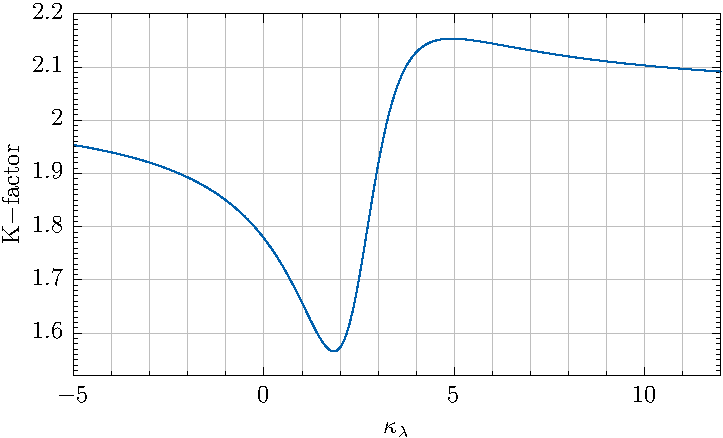
\includegraphics[width=0.65\textwidth]{plots/Kfactor.pdf}
%  \includegraphics[width=\textwidth]{plots/}
%    \caption{\label{fig:lambda_large_27}}
\caption{Variation of the NLO K-factor with the trilinear coupling at $\sqrt{s}=14$\,TeV.}
\label{fig:Kfacvariation}
\end{figure}


\begin{figure}[htb!]
\begin{minipage}[(a)]{0.5\textwidth}
\includegraphics[width=1.\textwidth]{plots/{NLO_cHHH_1_2_2.4_0_mHH-paper}.pdf}
\end{minipage}
\hfill
\begin{minipage}[(a)]{0.5\textwidth}
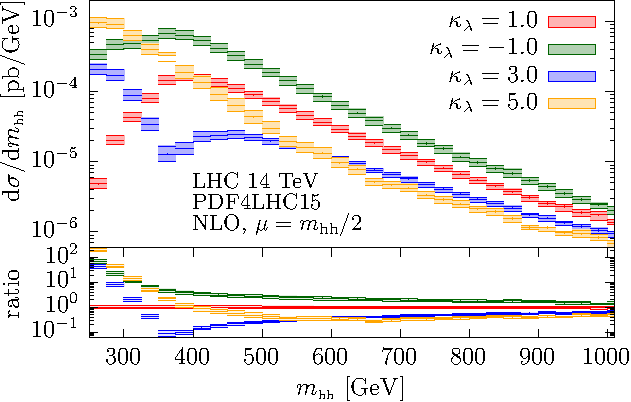
\includegraphics[width=1.\textwidth]{plots/NLO_cHHH_1_-1_3_5_mHH-paper.pdf}
\end{minipage}
\caption{Higgs boson pair invariant mass distributio	ns for various
  values of $\chhh$  at $\sqrt{s}=14$\,TeV. The uncertainty bands are from
  scale variations as described in the text.\label{fig:lambdavar14TeV}}
\end{figure}


\begin{figure}[htb!]
\begin{minipage}[(a)]{0.5\textwidth}
\includegraphics[width=1.\textwidth]{plots/{NLO_PP8_PH7_PH7D_cHHH_1_ptHH}.pdf}
\end{minipage}
\hfill
\begin{minipage}[(a)]{0.5\textwidth}
\includegraphics[width=1.\textwidth]{plots/{NLO_PP8_PH7_PH7D_cHHH_1_dRHH}.pdf}
\end{minipage}
\caption{The transverse momentum of one (any) Higgs boson and the $R$-separation between the two Higgs bosons are shown for the fixed-order NLO calculation and three shower setups, in 
the $\chhh=1$ case.}
\end{figure}
%\label{fig:lambdavar14TeV_pTHH_dRHH_showers}

\section{Conclusion}

\section*{References}

\bibliographystyle{iopart-num}
\bibliography{acat}{}

\end{document}


